% Diese Datei repräsentiert den Inhalt der Präsentation

% Titelseite
\begin{frame}[t,plain]
    \titlepage
\end{frame}

% table of contents
\section{Innføring}
\subsection*{Agenda}
\begin{frame}
    \tableofcontents
\end{frame}

\section{SQL}
\begin{frame}{Temaer}
\begin{itemize}
    \item Select
    \item Aggregation
    \item Joins
    \item Update
    \item Insert
    \item Delete
    \item Create and Drop Tables
    \item Datatyper
    \item Constraints
    \item Alt mulig
\end{itemize}
\end{frame}

\begin{frame}[fragile]{Select}
\begin{minted}{sql}
SELECT director, COUNT(*) as c -- Spalter
FROM movie                     -- Tabeller
WHERE country = "Dabendorf"    -- Betingelser
GROUP BY director              -- Gruppering etter spalter
HAVING c > 3                   -- Betingelser etter gruppering
ORDER BY c DESC                -- Sortering etter spalter 
LIMIT 3;                       -- Velg de første n output linjene
\end{minted}
\end{frame}

\begin{frame}[fragile]{Aggregation}
\begin{itemize}
    \item Count: Teller antall elementer
    \item Sum: Summerer verdier
    \item Avg: Gjennomsitt av verdier (tilsvarer count/sum)
    \item Min: Minimum
    \item Max: Maksimum
    \item Alle aggregasjonsfunksjoner ignorerer null verdier
\end{itemize}
\end{frame}

\begin{frame}[fragile]{Join}
\begin{minted}{sql}

\end{minted}
\end{frame}

\begin{frame}[fragile]{Update}
\begin{minted}{sql}

\end{minted}
\end{frame}

\begin{frame}[fragile]{Insert}
\begin{minted}{sql}

\end{minted}
\end{frame}

\begin{frame}[fragile]{Delete}
\begin{minted}{sql}

\end{minted}
\end{frame}

\begin{frame}[fragile]{Create Table}
\begin{minted}{sql}

\end{minted}
\end{frame}

\begin{frame}[fragile]{Drop Table}
\begin{minted}{sql}

\end{minted}
\end{frame}

\begin{frame}[fragile]{Datatyper}
\begin{minted}{sql}

\end{minted}
\end{frame}

\begin{frame}[fragile]{Constraints}
\begin{minted}{sql}

\end{minted}
\end{frame}

\begin{frame}[fragile]{Alt mulig}
\begin{minted}{sql}

\end{minted}
\end{frame}

\section{Relasjonsalgebra}
\section{ER-Diagrammer}
\section{Normalisasjon}
\section{Indekser (B-trær)}
\section{Transaksjoner}
\section{Alt mulig}

% Frames sind nicht Gleichzusetzen mit Seiten
% Ein Frame kann aus mehreren Seiten bestehen
% Ein Frame repräsentiert das, was ein Mensch als eine Seite ansieht, getrennt durch Animationseffekte wie das Aufklappen von weiteren Inhalten
% Ein Frame mit nur einer Aufzählung, die aus vier Unterpunkten besteht, die sich einzeln ausklappen ist also ein Frame, bestehend aus vier Seiten

% Beamer hat ebenfalls Sections und Subsections
% Sections werden im Header oben angezeigt und mit der Anzahl von \textit{Frames} oben als Punkte repräsentiert
%\section{Sichtbarkeiten}
%\subsection{Aufzählungen}
%
%% Der zweite Befehl hinter Frame fügt einen Extratitel auf der Folie ein
%% Man kann ihn auch weglassen
%\begin{frame}{Aufzählungen: Automatisches Aufklappen}
%% [<+->] Lässt alles einzeln aufklappen
%% [<+(2)->] stellt alternativ die Schritthöhe um, im Beispiel für zwei Unterpunkte auf einmal
%\begin{itemize}[<+->]
%    \item Aufzählungen funktionieren wie in klassischem LaTeX
%    \item Man kann einstellen, dass jeder Unterpunkt einzeln aufgeklappt wird
%    \item Hierdurch erhält jeder Unterpunkt einen einzelnen Frame
%    \item Hierfür muss nur hinter itemize ein Aufklappbefehl eingefügt werden
%\end{itemize}
%
%\end{frame}
%
%% <1-> Wird in x-tem (hier 1) Teilframe mit ausgeklappt
%\begin{frame}{Aufzählungen: Explizites}
%\begin{itemize}
%    \item<1-> Es ist möglich hinter jeden item-Befehl zu notieren, in der wievielten Teilseite dieses Frames es mit aufgeklappt wird.
%    \item<2-> In diesem Beispiel wird Punkt 1 allein aufgeklappt
%    \item<2-> Punkt 2 und 3 jedoch gemeinsam
%    \item<3-> Dieser hier wieder allein
%\end{itemize}
%
%\end{frame}
%
%% Der <a-b>-Befehl hat einen zweiten Parameter, welcher sagt, wann etwas verschwinden soll, wenn die Folie noch nicht fertig ist
%\begin{frame}{Aufzählungen: Sichtbar <von – bis>}
%\begin{itemize}
%    \item<1-2> Der genannte Befehl lässt auch Text wieder verschwinden, bevor der Befehl vorbei ist
%    \item<2-> In diesem Beispiel wird 
%    \item<2-> der erste Satz mit dem offenbaren des letzten Unterpunkts verschwinden
%    \item<3-> Lasset Punkt 1 verschwinden!
%\end{itemize}
%
%\end{frame}
%
%% \pause führt zu einer "Aufklapppause" und alles danach ist in einer neuen Folie
%\begin{frame}{Aufzählungen: Pausenbefehl}
%\begin{itemize}
%    \item Es gibt auch einen \texttt{pause}-Befehl
%    \item Mit ihm wird alles bis zu einem bestimmten Punkt aufgeklappt
%    \pause
%    \item Und alles danach in eine neue Folie gepackt
%\end{itemize}
%
%\end{frame}
%
%\subsection{Weitere Übergänge}
%% Pause-Befehl auch für allgemeine Textabschnitte oder sonstigen Kram nutzbar
%\begin{frame}{Sichtbarkeit von Text}
%Der Pause-Befehl ermöglicht es auch jedwede weitere Sachen erst nach und nach erscheinen zulassen.\pause~Dies ist zum Beispiel bei Fließtext der Fall.
%% Hinweis: ~ hinter einem Befehl erzeugt ein Leerzeichen, weil LaTeX sonst keines einfügen würde
%\end{frame}
%
%% Der Visible-Befehl sagt an, auf welchen Folien etwas sichtbar sein soll (analog zu <a-b>)
%\begin{frame}{Der Visible-Befehl}
%Auch der von-bis-Befehl hat für beliebige Sachen ein Pendant. Man kann mit dem \texttt{Visible}-Befehl und geschwungenen Klammern einen Bereich umrahmen, der nur von Teil-Seite x bis y sichtbar sein wird.
%
%\newLine % Der NewLine-Befehl wurde in der Präambel definiert und ist kein LaTeX-Standard. Er führt zu einem angenehmen Zeilenumbruch, der für Zentrierung der Inhalte einer Folie führt
%\visible<2-3>{
% $ G := (V, E)$ with $V$ a set of vertices and $E := \{ (a, b)$ and $(b, a)$ with $a, b \in V $ and $ a \neq b \} $
%
%}
%    
%\visible<3-3>{
%  \newLine
%  $ G = (\{1, 2, 3, 4, 5, 6\}, \{(1, 2), (2, 1),
%      (1, 3), (3, 1),
%      (1, 4), (4, 1), 
%      (2, 4), (4, 2), $ \\
%  \quad\quad $ (2, 5), (5, 2),
%      (2, 6), (6, 2),
%      (3, 4), (4, 3),
%      (3, 6), (6, 3),
%      (5, 6), (6, 5)\}) $
%}
%
%\visible<4>{
%  \begin{center}
%    Ich lasse nun all den Mathekram verschwinden
%  \end{center}
%}
%\end{frame}
%
%
%% Der Only-Befehl funktioniert ähnlich wie visible, gibt jedoch den Platz wieder an das nächste Element zurück
%\begin{frame}{Der Only-Befehl}
%Der Only-Befehl funktioniert wie Visible, aber gibt den Platz wieder frei\\
%\begin{center}
%  \begin{tabular}{cccccc}
%    $ \begin{tabular}{c}1: \\2: \\3: \\4: \\5: \end{tabular} $ &
%    $ \begin{bmatrix}-1.28078 \\0.280776 \\-1 \\-1.28078 \\2.28078 \end{bmatrix} $ &
%    $\rightarrow$ &
%    $ \begin{bmatrix}-1 \\1 \\-1 \\-1 \\1 \end{bmatrix} $ &
%    \visible<2>{$\rightarrow$} &
%    \visible<2>{\noindent\parbox[c]{2.5cm}{ $V_1 = \{1,3,4\}\\V_2 = \{2,5,6\}$}}
%  \end{tabular}\\
%  % Anmerkung: Die Mathematik dieser Folie ist nicht korrekt und dient Anschauungszwecken
%  
%  \only<1>{% Graph 1 ist auf der ersten Folie sichtbar
%    \myGraph
%  }
%  \only<2>{% Graph 2 ist auf der nächsten Folie an seiner Stelle sichtbar
%    \myGraphCorrect
%  }
%\end{center}
%\end{frame}
%
%\section{Sonstiges}
%
%\subsection{Textblöcke}
%
%\begin{frame}
%    \frametitle{Textblöcke}
%    
%    Es gibt standardmäßig drei Sorten von Textblöcken in rot, grün und blau, die man sympathisch aussehend in Präsentationen einfügen kann. Ihre Farben sind wie in \LaTeX~ üblich änderbar und weitere hinzufügbar. Wenn man weiß wie. \alert{Ahahahamumumu}.
%    
%    % Der zweite Parameter (hier Remark) legt die Überschrift fest
%    \begin{block}{Remark}
%    Ihre Namen sind \texttt{block}, \texttt{alertblock} und \texttt{examples}
%    \end{block}
%    
%    \begin{alertblock}{Important theorem}
%    Französisch ist eine schrecklich anstrengende Sprache.
%    \end{alertblock}
%    
%    \begin{examples}
%    Un bel avion est un avion qui vole bien.
%    \end{examples}
%\end{frame}
%
%\subsection{Zweispaltiges Layout}
%\begin{frame}
%    \begin{columns}
%    
%    \column{0.5\textwidth}
%    Darstellung in zwei Spalten ist \textit{natürlich} möglich.
%    $$P\stackrel{?}{=} NP$$
%    \begin{itemize}
%    \item Präsentationsfanatiker können auch hier
%    \item die Spalten nacheinander erscheinen lassen
%    \item Aber wer macht sowas?
%    \end{itemize}
%    
%    \pause
%    \column{0.5\textwidth}
%    Hierfür nutzt man den \texttt{column}-Befehl und setzt die Breite der Columns entsprechend fest. Hier ist das eine 50-50-Aufteilung.
%    \end{columns}
%
%\end{frame}
%
%% Ein komplexeres Beispiel
%% noframenumbering führt dazu, dass eine Seite nicht mit in die Seitenzahlen hinein gezählt wird
%% Wer braucht sowas? Ingen vet
%\begin{frame}[noframenumbering]
% \begin{columns}
%    \begin{column}{0.52\textwidth}
%	\begin{table}
%    	\begin{tabular}{l|l|c|c|}
%    	\multicolumn{2}{c}{}&\multicolumn{2}{c}{Tatsächlich}\\
%    	\cline{3-4}
%    	\multicolumn{2}{c|}{}&Positiv&Negativ\\
%    	\cline{2-4}
%    	\multirow{2}{*}{Vorhergesagt}& Positiv & $TP$ & $FP$\\
%    	\cline{2-4}
%    	& Negativ & $FN$ & $TN$\\
%    	\cline{2-4}
%    	\end{tabular}
%	    \caption{Konfusionsmatrix}
%	    \label{tab:confusion-matrix}
%    \end{table}
%    \end{column}
%    
%    \begin{column}{0.52\textwidth}
%    \begin{center}
%        ${\displaystyle Precision = \frac{TP}{TP+FP} } $\\[5mm]
%        ${\displaystyle Recall = \frac{TP}{TP+FN} } $\\[5mm]
%        ${\displaystyle F_1 = \frac{2\cdot Precision\cdot Recall}{Precision + Recall} } $
%    \end{center}
%    \end{column}
% \end{columns}
%\end{frame}
%
%\subsection{Bilder einfügen}
%\begin{frame}{Graphiken einfügen wie sonst auch}
%    \begin{figure}
%        \centering
%        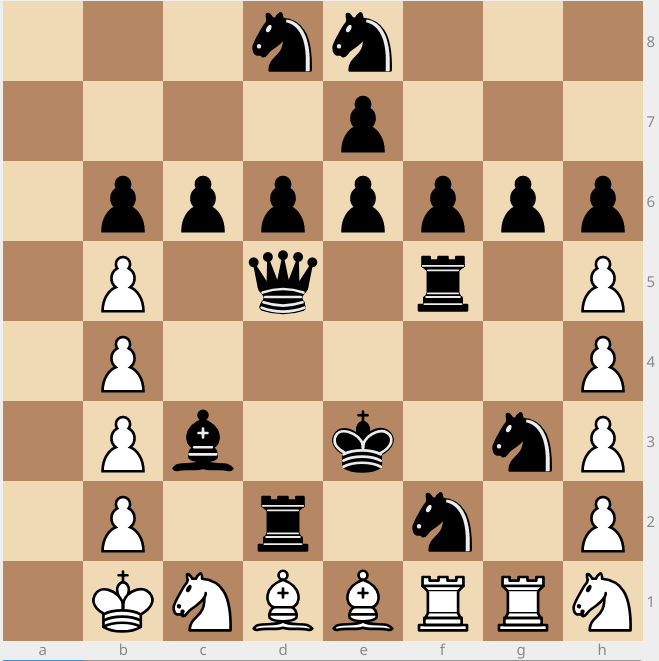
\includegraphics[height = 4.9cm]{puzzle.png}
%        \caption{Schwarz am Zug, Matt in 5}
%        \label{fig:chesspuzzle}
%    \end{figure}
%\end{frame}


\section*{Slutt}
\begin{frame}
\begin{center}\textbf{Takk for oppmerksamheten\\Lykke til med eksamenen}\end{center}  
\end{frame}